\documentclass[11pt,a4paper,ngerman]{article}
\usepackage[bottom=2.5cm,top=2.5cm]{geometry} 
\usepackage{babel}
\usepackage[utf8]{inputenc} 
\usepackage[T1]{fontenc} 
\usepackage{ae} 
\usepackage{amssymb} 
\usepackage{amsmath} 
\usepackage{graphicx}
\usepackage{fancyhdr}
\usepackage{fancyref}
\usepackage{listings}
\usepackage{xcolor}
\usepackage{paralist}

%%\usepackage[pdftex, bookmarks=false, pdfstartview={FitH}, linkbordercolor=white]{hyperref}
\usepackage{fancyhdr}
\pagestyle{fancy}
\fancyhead[C]{Höhere Algorithmik}
\fancyhead[L]{Übung Nr. 4}
\fancyhead[R]{WS 2011/12}
\fancyfoot{}
\fancyfoot[L]{}
\fancyfoot[C]{\thepage$\,$ von \pageref{LastPage}}
\renewcommand{\footrulewidth}{0.5pt}
\renewcommand{\headrulewidth}{0.5pt}
\setlength{\parindent}{0pt} 
\setlength{\headheight}{15pt}

\author{Tutor: Lena Schlipf}
\date{}
\title{Max Wisniewski , Alexander Steen}

\begin{document}

\lstset{language=Java, basicstyle=\ttfamily\fontsize{10pt}{10pt}\selectfont\upshape, commentstyle=\rmfamily\slshape, keywordstyle=\rmfamily\bfseries, breaklines=true, frame=single, xleftmargin=3mm, xrightmargin=3mm, tabsize=2, mathescape=true}

\maketitle
\thispagestyle{fancy}

%% ------------------------------
%%       Aufgabe 1
%% ------------------------------
\section*{Aufgabe 1}

Sei $P$ eine Menge von $n$ Punkten in der Ebene, In der Vorlesung haben Sie einen Algorithmus kennengelernt, der ein engstes Paar von $p$ in Zeit $O \left( n \log n \right)$ bestimmt. Dabei haben wir angenommen, dass alle $x$-Kooridnate in $P$ verschieden sind. Zeigen Sie, wie man den Algorithmus anpassen kann, damit wir diese Annahme nicht mehr benötigen. Die Laufzeit soll immer noch $O\left( n \log n \right)$ betragen.\\

\textbf{Lösung:}

Das Problem an dieser Stelle ist, dass wir nach dem Algorithmus die Menge $P$ in 2 Teile spalten $R_L = \{ p \in P \; | \; p_x < q_x\} \cup \{q\}$ und $R_R = \{ p \in P \; | \; p_x < q_x\}$, wobei $q$ der Median der $x$-Koordinaten ist. Nun würden wir aber alle Elemente, die die selbe $x$ - Koordinate des Medians haben, nicht mit betrachten. Im schlimmsten Fall würden wir also alle Punkte paarweise betrachten müssen, weil in $R_L$ nur $q$ liegt und $R_R = \emptyset$ gilt, wenn alle Elemente die selbe $x$ - Koordinate haben. Da innerhalb dieser Mengen kein Abstand existiert, muss $\delta = \infty$ gelten. Würden wir nur 10 Elemente paarweise vergleichen, würden wir den geringsten Abstand unter umständen nicht finden.\\

Dieses Problem können wir lösen indem wir uns die Optimierung des Algorithmuses aus der VL betrachten und uns ansehen, was bei gleichen Elementen passiert.\\
Wir haben die Punkte nach $x$ - Koordinaten vorsortiert. Danach geben wir nur noch Zeiger für ein minimales Element und ein Zeiger für ein maximales Element weiter. Um den $x$ Median zu finden müssen wir nun nur bei $\frac{min + max}{2}$ nachsehen und haben $q$. Nun teilen wir die Punktmenge in 2 gleichgroße Teile, indem wir als Zeiger $(min, \frac{min+max}{2})$ und $(\frac{min+max}{2}+1,max)$ weiter geben. So haben wir nicht nur die kleinere und größeren in 2 Teile gespalten, sondern auch noch die gleichen. Hier geraten wir also nicht in die Verlegenheit einige Punkte nicht zu betrachten. Sonst bleibt der Algorithmus gleich.\\

Als Laufzeit ergibt sich exakt die selbe, da wir eigentlich nichts gemacht habe. Wir haben die Vorverarbeitungszeit $O(n \log n)$ und pro Schritt benötigen wir wieder $T(n) = 2 T(\frac{n}{2}) + O(n)$. Da wir beim Teilen nicht mehr tun müssen als vorher. Dies ergibt wieder eine Laufzeit von $O(n \log n)$

\pagebreak
%% ------------------------------
%%       Aufgabe 2
%% ------------------------------
\section*{Aufgabe 2}

Sei $G = \left( V, E \right)$ ein Gittergraph mit $n$ Zeilen und $n$ Spalten. Formal heißt das:\\
$V = \left\{ \{ (i,j), (i' , j') \} | \left| i - i' \right| + \left| j - j' \right| = 1 \right\}$. Desweiteren sei jeder Knoten $v \in V$ mit einer Zahl $x_v \in \mathbb{R}$ beschriftet, so dass die $x_v$ paarweise verschieden sind. Ein \emph{lokales Minimum} von $G$ ist ein Knoten, dessen Beschriftung kleiner ist als die Beschriftung seiner Nachbern.

\begin{enumerate}[\bfseries (a)]


%% ------------------------------
%%      	a)
%% ------------------------------
\item Zeigen Sie, dass immer ein lokales Minimum existiert.\\

\textbf{Lösung:}\\
Der Graph $G$ hat nach Definition $n^2$ viele Knoten. Dies bedeutet insbesondere, dass $W = \{ x_v \; | \; v \in V \}$ eine endliche, nicht-leere Menge ist.\\
Für jede endliche, niicht-leere Teilmenge über einer total geordneten Grundmenge gilt, dass diese eine (globales) Minimum und Maximum besitzt\footnote{Wie in Mafi I gezeigt wurde}. Nun ist $\mathbb{R}$ eine total geordnete Menge und $W \subset \mathbb{R}$. Damit besitzt $W$ ein (globales) Minimum.\\

Sei $m \in M$ nun der Knoten mit $x_m = \min W$. Da gilt, dass die Elemente aus $W$ alle paarweise verschieden sind, gilt ins besonderen, dass\\
$\forall v \in V \; : \; x_v \leq x_m$ oder $\forall v \in V \setminus \{m\} \; : \; x_v < x_m$.\\

Dies gilt insbesondere auch für die Nachberknoten von $m$. Damit ist $m$ auch sowohl \emph{globales Minimum} als auch \emph{lokales Minimum} in diesem Graphen.


%% ------------------------------
%%       b)
%% ------------------------------
\item Der folgende Algorithmus heißt \emph{lokale Suche}: Beginne bei einem beliebigen Knoten $v \in V$. Falls ein $v$ ein \emph{lokales Minimum} ist, sind wir fertig. Ansonsten hat $v$ einen Nachbern $w$ mit $x_w < x_v$ (wenn es mehr als einen solchen Nachbern gibt, wählen wir denjenigen mit dem kleinsten $x_w$). Gehe zu $w$ und wiederhole, bis ein lokales Minimum erreicht ist.\\

Zeigen Sie, dass lokale Suche im schlimmesten Fall $\Omega (n^2)$ viele Schritte benötigt.\\

\textbf{Lösung:}\\
Um diese Laufzeit zu erreichen Konstruieren wir uns einen Fall, indem bei gegebenem $v\in V$ der Algorithmus jedes (i-te) Element $w in V$ besuchen muss, wobei $i\in \mathbb{N}$ konstant ist.\\

Unsere Konstruktion sieht wie folgt aus: Wir starten bei $v$ in der linken, oberen Ecke $i = j = 0$. Nun wählen wir Schlangenlinien durch unseren Pfad, so dass wir immer eine Zeile überspringen (am Rand nur 1 Element berühren). Die Knoten entlang dieses Pfades sind immer um 1 kleiner als der Vorgänger. (Wir starten bei $x_{0,0} = n^2$. Die Knoten aus den frei gelassenen Ebenen, wählen wir so, dass wir sie nicht betreten, groß genug und beliebig ($> n^2$).

Asl Folge erhalten wir so : $x_{0,0} > x_{0,1} > ... > x_{0,n} > x_{1,n} > x_{2,n} > x_{2,n-1} > ... > x_{2,0} > x_{3,0} > ...> x_{n,n}$
(Wenn $n$ gerade ist, sonst $x_{0,n}$). Der Weg sieht also folgender Maßen aus:

\begin{figure}[h!]
\centering
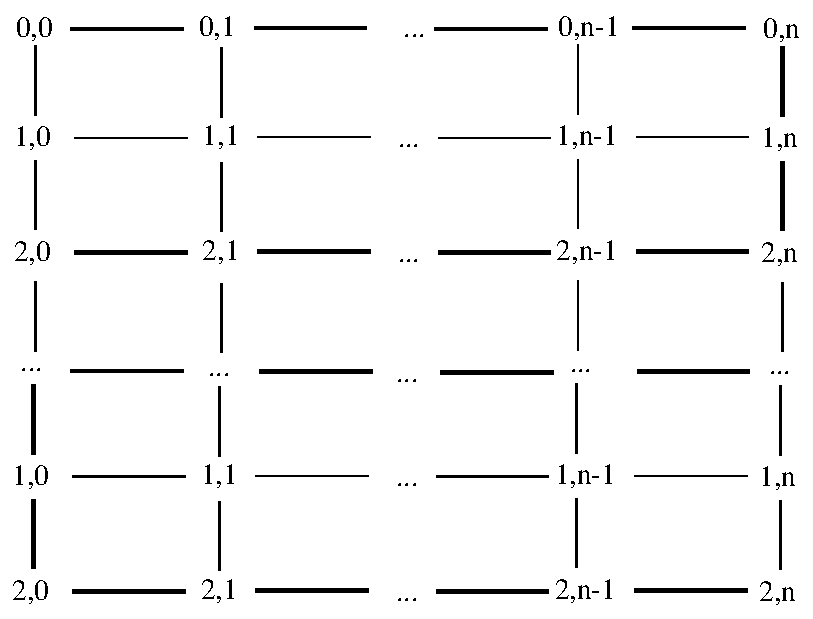
\includegraphics[scale=0.7]{a2_worst_case.pdf}\\
Stellt einen Pfad dar, der $\Omega (n^2) $ viele Knoten besucht.
\end{figure}

Wir berühren hier $\frac{n^2}{2} + \frac{n}{2}$ Knoten. Diese kommen zustande indem wir jede zweite Spalte komplett durchgehen und jede andere nur ein Element betrachten. Auf jedem dieser Felder haben wir 4 Vergleiche gemacht. Dies lässt uns bei einer Laufzeit von $\Omega (n^2)$.

%% ------------------------------
%%       c)
%% ------------------------------
\item Zeigen Sie, wie man ein lokales Minimum in $O (n)$ Zeit finden kann. Begründen Sie Korrektheit und Laufzeit Ihres Algorithmus.

\textbf{Lösung:}\\
Die Idee dieser Lösung sieht wie folgt aus:\\
Wir legen in jedem Schritt ein Kreuz über das Feld, so dass es das gesammte Gitter in 4 (in etwa) gleichgroße Teile zerlegt. Als nächstes suchen wir uns das Minimum dieser $2 \cdot n - 1$ Elemente, die auf dem Kreuz liegen. Von dem Knoten des Minimums aus, betrachten wir die beiden Nachbern, die nicht in dem Streifen liegen (wahlweise auch alle, da kein Nachber auf dem Streifen kleiner sein kann). Ist keines der Elemente kleiner, so haben wir lokales Minimum. Sonst gehen wir in Richtung des kleineren Nachberns.
Damit haben wir ein $\frac{3}{4}$ des Quadrates weggeworfen und müssen nur nach das verbleibende Viertel mit den Maßen $\frac{n}{2} \times \frac{n}{2}$ weiter machen.

\begin{figure}[h!]
\centering
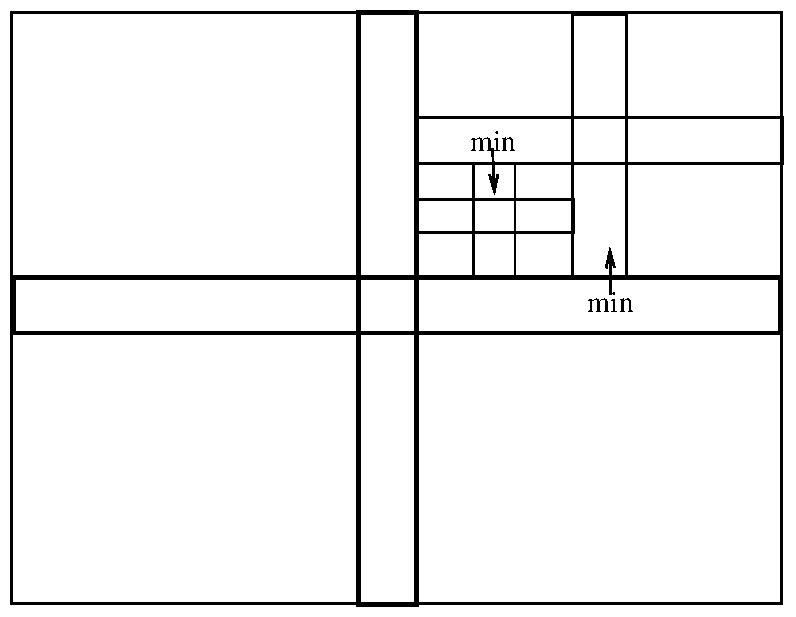
\includegraphics[scale=0.7]{local_min.pdf}\\
Ein Grid das die Aufteilung rekursiv Darstellt.
\end{figure}

\pagebreak

\textbf{Korrektheit:}\\
Für die Korrektheit zeigen wir, dass ein \emph{lokales Minimum} im eingeschränkten Viertel liegen muss (außer wir haben schon eins im Streifen gefunden gefunden).\\

Betrachten wir für den Beweis das Porgram aus \emph{b)}. Wir wählen als Startknoten des Algorithmus das Minimum unseres Streifen $y$. Wir wissen, dass der Algorithmus entlang der kleinere Elemente läuft. Nun wissen wir, dass er immer ein \emph{lokales Minimum} finden muss (Sollte dies nicht gegeben sein, nehmen wir die Quellensuche auf POSETs, wie sie in Mafi I gezeigt wird, da diese analog abläuft).
Im ersten Schritt betritt der Algorithmus unser ausgewählte Rechteck nach Konstruktion.\\

Nun wissen wir, dass die Folge $(a_n)_{n \in \mathbb{N}}$ der besuchten Knoten eine monoton fallende sein muss, mit $a_0 = m$, da jeder folgende Wert kleiner sein muss (nach Algorithmus). Da nun aber für das Kreuz $K$ gilt, dass\\
$\forall k \in K \setminus \{m\} \; : \; k > m$\\
und für die Folge, dass\\
$\forall n \in \mathbb{N} \; : \; a_n < m$, was direckt aus der monotonie folgt.
$$
\Rightarrow \forall k \in K \; \forall a \in (a_n)_{n \in \mathbb{N}} \; : \; k > a \Rightarrow K \cap (a_n)_{n \in \mathbb{N}} = \{m\}
$$
Da wir nach Konstruktion aber nicht über $m$ zurücklaufen können, da wir nur in Richtung eines echt kleineren gehen können, also keine Schleifen bilden können. Die Folge muss also auf ein Element innerhalb unsere eingeschränkten Quadrates liegen.\\
\mbox{} \hfill $\square$

\textbf{Laufzeit:}\\
Um das Minimum von $2n-1$ Elementen zu finden benötigen wir $2n-2$ Vergleiche\footnote{gezeigt in ALP3}. Von da aus brauchen wir noch 2 Vergleiche um den Teil des kleineren Nachbern zu ermitteln. Danach fahren wir auf den halbierten Zeilen und Spalten fort (sollten wir zu wenig haben für die Hälfte, nehmen wir uns weitere Elemente aus dem Streifen, dies macht es nicht falsch, aber leichter zu analysieren).

$$
\Rightarrow T(n) = \left\{
\begin{array}{lr}
c_1 n &, n < 4 \text{(egal solange konstant)}\\
T(\frac{n}{2}) + c_2 n &, sonst
\end{array}
\right.
$$
Mit $c_1, c_2 \in \mathbb{R}^+$ konstant.
\end{enumerate}

Dies können wir nun mithilfe des Mastertheorems abschätzen:\\
$a=1, b=2, f(n) = c_2 n$\\
Wir prüfen den 3. Fall des Theorems:\\
$f(n) = c_2 \cdot n = \Omega (n^{0 + 1})= \Omega (n^{\log_1 2 + 1})$, mit $\varepsilon = 1$\\
und\\
$a f(\frac{n}{b}) = f(\frac{n}{2}) = \frac{1}{2}n \leq c \cdot n$, mit $c = \frac{3}{4}$\\
Damit sind die Bedingungen für den 3. Fall des Mastertheorems erfüllt und es gilt:
$$
\Rightarrow T(n) = \Theta ( n)  
$$\\

Damit haben wir gezeigt, das wir ein \emph{lokales Minimum} in $O(n)$ finden können.

%% ------------------------------
%%       Aufgabe 3
%% ------------------------------
\section*{Aufgabe 3}

Für eine gegebene Folge $M_1 , M_2, ... , M_n$ von $n$ Matrizen ist das \emph{Matrizenkettenprodukt} $M_1 \cdot M_2 \cdot \cdots \cdot M_n$ zu berechnen. Die Matrizen haben dabei verschiedene Dimensionen. $M_1$ ist eine $p_1 \times p_2$ Matrix, $M_2$ ist eine $p_2 \times p_3$ Matrix usw.\\

Um eine $a\times b$ Matrix mit einer $b \times c$ Matrix zu multiplizieren, benötigen wir bekanntlich $acb$ Multiplikationen und $ac\left( b - 1 \right)$ Additionen, also insgesammt $ac \left( 2b - 1\right)$ Additionen, also insgesamt $ac\left( 2b - 1\right)$ elementare Operationen.

\begin{enumerate}[\bfseries (a)]


%% ------------------------------
%%       a)
%% ------------------------------
\item Bezeichne mit $P[i,j]$ die Kosten für eine optimale Klammerung des Matrizenkettenprodukts $M_i \cdot \cdots \cdot M_j \; ( 1 \leq i \leq j \leq n)$. Unser Ziel ist, $P[1,n]$ zu berechnen. Finden Sie eine geeignete Rekursionsgleichung für $P[i,j]$.\\

\textbf{Lösung:}
$$
\begin{array}{lcrcl}
\forall 1 \leq i = j \leq n &\; : \;& P[i,j] &=& 0\\
&& P[i,j] &=& \underset{a \in (i,j)}{\min} P[i,a] + P[a+1,j] + p_i \cdot p_{j+1} \cdot (2 \cdot p_{a+1} - 1)
\end{array}
$$

Da immer gilt, dass $i \leq j$ ist, liegt unser Anker auf der Diagonalen. Wir brauchen nur den oberen oder unteren Teil der Matrix auszufüllen (je nachdem auf welcher achse $i$ und $j$ steht).\\

Diese Gleichung sucht immer Schrittweise nach der besten Multiplikation. Wir teilen die Menge der Matrizen in 2 Hälften und suchen uns die beste lokale Partitionierung herraus, wenn wir die kosten für die Addition der beiden Ergebnisse mit drauf rechnen. In $P[1,n]$ steht danach das globale Maximum.

%% ------------------------------
%%		b)
%% ------------------------------
\item Benutzen Sie Ihre Rekursion, um Pseudecode für einen Algorithmus anzugeben, welcher die optimalen Kosten $P[1,n]$ bestimmt. Analysieren Sie Laufziti und Platzbedarf.\\

Der Pseudocode sieht, wie folgt aus:

\begin{lstlisting}[language=Pascal, numbers=right]
for i := 1 to n do
	P[i,i] := 0;
	Back[i,j] = null;	//Marker fuer das Ende
for j := 1 to n do
	for i := 1 to j do
		wa := $\infty$ ;// Maximaler Wert bisher
		a := null;	// Voraenger mit dem groessten Wert
		for x := i to j do
			mom = P[i,x] + P[x+1,j] + p[i]*p[j+1]*(2*p[x+1]-1);
			if mom > wa then
				wa = mom;
				a := x;
		P[i,j] = wa;
		Back[i,j] = a;
\end{lstlisting}

\pagebreak

\textbf{Platzbedarf:} Für diesen Algorithmus legen wir, wenn wir es einfach machen ein 2 Dimensionales Array, der Größe $n \times n$ an. Da wir aber in jedem in Zeile $i$ nur jeweils $i$ der Einträge brauchen (Start bei 1) könnten wir es auch optimieren, dass wir unterschiedlich Lange Arrays in das erste packen. Da wir aber damit immer noch $\underset{i=1}{\overset{n}{\sum}} i$ Einträge brauchen, verbleiben wir bei einem Speicherplatzbedarf von $\Theta (n^2)$.\\

\textbf{Laufzeit:} Als Laufzeit für den Algorithmus schauen wir uns an, wie viele Operationen wir pro benutzem Feld haben.\\
Nun müssen wir aber Pro Feld nicht 1 annehmen, sondern haben pro Feld $i-j$ $c$ konstante Operationen. Dies ergibt die Formel:
$$
T(n) = \sum_{j=0}^{n} \sum_{i=0}^{j} (i-j) \cdot c = \frac{1}{6} cn \cdot (n + 1) \cdot (n + 2)
$$ 
Das gibt uns eine Laufzeit von $\Theta(n^3)$, die allerdings sehr gute Konstanten besitzt. (Das c bewegt sich im Bereich von $\approx 6$ elementar Operationen).

%% ------------------------------
%%      	c)
%% ------------------------------
\item Erweitern Sie Ihren Algorithmus so, dass er auch eine optimale Klammerung ausgibt.\\

Im in \emph{b)} beschriebenen Algorithmus haben wir schon ein Feld \emph{Back} angelegt, indem wir für jedes Feld gespeichert haben, wo wir weiter geklammert haben. Anahnd dieser Information können wir den optimalen Weg rekonstruieren (Wir habe uns für eine reine Rekursion entschieden, da sie am leichtesten verständlich ist):

\begin{lstlisting}[language=Pascal]
OptimaleKlammerung(i,j)
	if( i = j)
		return "M_" + i;
	a = Back[i,j];
	links = OptimaleKlammerung(i,a);
	rechts = OptimaleKlammerung(a+1,j);
	return "(" + links + ") * (" + rechts + ")";
\end{lstlisting}

Sollten wir nun eine optimale Klamerung benutzen wollen zum ausrechnen, so geben wir keine Strings zurück, sondern Matrizen und beim zusammensetzten (letzem return) multiplizieren wir die Matrizen einfach.

\pagebreak

%% ------------------------------
%%      	d)
%% ------------------------------
\item Implementieren Sie ein Programm, das eine optimale Klammerung für die Matrizenmultiplikation bestimmt und die Multiplikation durchführt. Vergleichen SIe Ihr Programm mit einer naiven Implementierung, welche die Matrizen von links nach rechts multipliziert.

\begin{description}

\item{\bfseries Implementierung:}

\begin{lstlisting}
public static Matrix naive_ketten_multiplikation(Matrix[] matrices){
	...
	Matrix erg = matrices[0];
	for(int i = 1; i < matrices.length; i++){
		erg = Matrix.matmult(erg, matrices[i]);
	}
	return erg;
}
\end{lstlisting}
Wir gehen unser Feld von Matrizen durch und multiplizieren diese der Reihe nach auf.\\


\begin{lstlisting}
public static Matrix kettenMultiplikation(Matrix[] matrices){
	// ... Fehler / kleine Werte etc.
	int n = matrices.length;
	dyn = new int[n][n];
	back = new int[n][n];
	
	for(int i = 0; i < n; i++){
		dyn[i][i] = 0;
		back[i][i] = -1;
	}
	for(int j = 0; j< n; j++){
		for(int i = 0; i<j; i++){
			int acc = Integer.MAX_VALUE;
			int a = 0;
			for(int x=i; x<j; x++){
				int mom = dyn[i][x] + dyn[x+1][j] + matrices[i].getColumnDimension() * matrices[j].getRowDimension()*(2*matrices[x].getRowDimension());
				if(mom < acc){
					acc = mom;
					a = x;
				}
			}
			dyn[i][j] = acc;
			back[i][j] = a;
		}
	}
	matToMult = matrices;
	return multByReverse(0, n-1);
}
\end{lstlisting}

Wir gehen genau wie in \emph{b)} beschrieben vor. Der Algorithmus ist nur auf JAVA angepasst. Wir haben uns dafür entschieden in der naiven und in der dynamischen die Schulmethode der Matrixmultiplikation zu verwenden, da Strassen für nicht quadratische Matrizen, die keine Zweierpotenzdimensionen haben, zu aufwendig zu implementieren ist. (Man könnte die Matrizen auf quadratische, zweierpotenz Matrizen erweitern, indem man 0en anhängt und danach die Dimension, die man erwartet wieder herstellt)

\pagebreak

\begin{lstlisting}
private static Matrix multByReverse(int i, int j){
	if(i == j){
		return matToMult[i];
	}
	int a = back[i][j];
	return Matrix.matmult(multByReverse(i,a), multByReverse(a+1,j));
}
\end{lstlisting}

Diese Methode funktioniert, wie in \emph{c)} beschrieben. Wenn wir ein und die selbe Matrix haben, werden wir diese zurück geben. Sonst suchen wir uns den gespeicherten Wert, nehmen an dieser Stelle die Teilung vor, multiplizieren Rekursiv die Matrizen. Wenn diese Methoden zurückkehren, werden wir die Ergebnisse multiplizieren.

\item{\bfseries Testläufe:}\\
Die Testläufe laufen über eine Anzahl $n$ (bei uns auf 100 gesetzt) random generierte Matrizen (die Dimension ist auf 200 begrenzt).\\
Wenn der Parameter ('-o') angegeben wurde, so werden diese Matrizen alle ausgegeben werden. Am Ende werden die Zeiten für die Multiplikation der naiven und der dynamischen Lösung ausgegeben.\\


Unsere Testläufe haben erstens ergeben, dass die Multiplikation das selbe Ergebnis liefert. (Getestet mit Parameter '-o'). Von der Laufzeit her betrachtet haben wir je nachdem, wie schlecht die naive Klammerung ist, einen minimalen Geschwindigkeitsverlust (lag bei wenigen ms drunter) bis zu einem Speed-Up von 15. Im Schnitt konnten wir beobachten, dass die dynamische Implementierung etwa 8 mal so schnell war.
\end{description}

\end{enumerate}

\label{LastPage}

\end{document}
